\chapter{Concepts and Techniques}

This chapter introduces the concepts and techniques used in the report. We first review regular expressions, finite automata, the Glushkov construction, and BST-like distributions. We then discuss SIMD parallelism and its role in regular expression matching. Finally, we introduce tools from analytic combinatorics and Monte Carlo simulation, which are used to analyze asymptotic recurrences and estimate distributions. Some functional-analytic tools are introduced later in Chapter \ref{chap:length-of-longest-literals}, when they are needed for the longest literal problem.

\section{Regular expressions}

% Regular expressions, finite automata, Glushkov construction, BST distribution.

A \textit{regular expression} is a string that describes a set of strings according to certain syntax rules. Formally, given a finite alphabet $\Sigma$, the set of regular expressions over $\Sigma$ is defined inductively. The base cases consist of the empty set $\emptyset$, the empty word $\epsilon$, and literal characters $a \in \Sigma$. More complex expressions are constructed using three fundamental operators: alternation ($\mid$), concatenation (implicit or $\cdot$), and the Kleene star ($*$). Semantically, a regular expression $E$ maps to a formal language $\mathcal{L}(E) \subseteq \Sigma^*$ via the following structural rules:
\begin{align*}
   & \mathcal{L}(\emptyset)     = \emptyset, \quad \mathcal{L}(\epsilon) = \{\epsilon\}, \quad \mathcal{L}(a) = \{a\}, \\
   & \mathcal{L}(E_1 \mid E_2)     = \mathcal{L}(E_1) \cup \mathcal{L}(E_2),                                           \\
   & \mathcal{L}(E_1 \cdot E_2) = \{ xy \mid x \in \mathcal{L}(E_1), y \in \mathcal{L}(E_2) \},                        \\
   & \mathcal{L}(E^*)            = \bigcup_{n \ge 0} \mathcal{L}(E)^n.
\end{align*}
Any language generated by these rules is called a regular language. In practice, regular expressions are often extended with additional operators, such as the plus operator ($+$), which denotes one or more repetitions, the question mark operator ($?$), which denotes zero or one occurrence, and the bounded repetition operator ($\{m,n\}$), which denotes between $m$ and $n$ occurrences. These extensions preserve the class of regular languages because they can be expressed using the fundamental operators: $E^+ = E \cdot E^*$, $E? = \epsilon \mid E$, and $E^{\{m,n\}} = E^m \cdot (E?)^{n-m}$.

A fundamental result in formal language theory is that the expressive power of regular expressions is identical to that of \textit{finite automata}, which provide an operational point of view \cite{sipser2012introduction}. A finite automaton has a set of states, a distinguished start state, and a set of accepting states. Transitions between states are triggered by input symbols. The formal definition is as follows.

\begin{definition}
  A (non-deterministic) finite automaton (NFA) is a quintuple $(\Sigma, Q, q_0, F, \delta)$ where
  \begin{itemize}
    \item $\Sigma$ is a finite alphabet of input symbols,
    \item $Q$ is a finite set of states,
    \item $q_0 \in Q$ is the start state,
    \item $F \subseteq Q$ is the set of terminal states, and
    \item $\delta: Q \times \Sigma \to 2^Q$ is the transition function.
  \end{itemize}

  The automaton is a deterministic finite automaton (DFA) if $\delta(q,a)$ is a singleton for every $q\in Q$ and $a\in\Sigma$.
\end{definition}

\begin{example}
  Let $\Sigma = \{a,b\}$. The regular expression $E = (b \mid ab)^*(\epsilon \mid a)$ consists of all strings over $\Sigma$ that do not contain two consecutive $a$'s. The corresponding DFA is shown in Figure \ref{fig:dfa_no_aa}.
\end{example}

\begin{figure}[htbp]
  \centering
  \begin{tikzpicture}[
    shorten >=1pt,
    node distance=3cm,
    on grid,
    auto,
    >={Stealth[round]} % Clean, modern arrowheads
    ]
    % State definitions
    \node[state, initial, accepting] (q0) {$q_0$};
    \node[state, accepting, right=of q0] (q1) {$q_1$};
    \node[state, right=of q1] (q2) {$q_2$};

    % Transitions
    \path[->]
    (q0) edge [loop above] node {b} (q0)
    edge [bend left]  node {a} (q1)
    (q1) edge [bend left]  node {b} (q0)
    edge              node {a} (q2)
    (q2) edge [loop above] node {a, b} (q2);
  \end{tikzpicture}
  \caption{DFA recognizing strings over $\{a,b\}$ that do not contain $aa$.}
  \label{fig:dfa_no_aa}
\end{figure}

Finite automata are basic data structures for regular expression matching. The Glushkov construction \cite{glushkov1961abstract} used by Hyperscan is a well-known algorithm that converts a regular expression into an equivalent NFA. It has several useful properties: it has no $\epsilon$-transitions, the number of states is one more than the number of symbols in the regular expression, and all incoming transitions to a given state read the same letter.

Average-case analysis of algorithms on regular expressions requires a probability distribution over regular expressions. More precisely, we use a distribution over syntax trees of regular expressions, which are rooted ordered trees representing the structure of a regular expression. The syntax tree of a regular expression is not unique: for example, $abc$ has two syntax trees, each corresponding to a different bracketing of the concatenation operator.

It is known that the uniform distribution over syntax trees of regular expressions over a two-letter alphabet tends to generate reduced syntax trees of sizes bounded by 80 \cite{koechlin2021analysis}. This suggests that the uniform distribution is not a good model for analyzing the average-case complexity of algorithms on large regular expressions. Instead, we use a generalized family of generators over binary search trees (BST), commonly called BST-like distributions. A tree of size $n$ is generated as follows. If $n=1$, a literal is generated uniformly at random. If $n>1$, a node is generated with probability $u$ or $v$ for the concatenation or alternation operator, respectively, and with probability $1-u-v$ for the Kleene star operator. The subtrees are then generated recursively with sizes summing to $n-1$. The formal definition is given below, using a probability function $p:\T \to [0,1]$ that maps a syntax tree to its probability of being generated, such that $\sum_{|T| = n} p(T) = 1$.

\begin{definition}[BST-like distributions]
  \label{def:bst-like-distribution}
  Let $u$ and $v$ be parameters in $[0,1]$ with $u + v < 1$. The function $p:\T \to [0,1]$ is defined inductively as follows.
  \begin{enumerate}
    \item $\sum\limits_{c\in\Sigma}p(c) = 1$,
    \item $p\left(\vcenter{\hbox{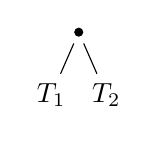
\begin{tikzpicture}[level distance=8mm, sibling distance=7mm, edge from parent/.style={draw, shorten <=1mm}]
                  \node[circle, draw, fill=black, minimum size=1mm, inner sep=0pt] {}
                  child { node {$T_1$} }
                  child { node {$T_2$} };
                \end{tikzpicture}}}\right) = \dfrac{u}{n-2} p(T_1)p(T_2)$, where $|T_1| + |T_2| = n-1$.
    \item $p\left(\vcenter{\hbox{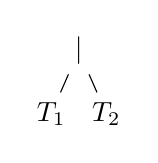
\begin{tikzpicture}[level distance=8mm, sibling distance=7mm]
                  \node{$\mid$}
                  child { node {$T_1$} }
                  child { node {$T_2$} };
                \end{tikzpicture}}}\right) = \dfrac{v}{n-2} p(T_1)p(T_2)$, where $|T_1| + |T_2| = n-1$.
    \item $p\left(\vcenter{\hbox{\begin{tikzpicture}[level distance=8mm, sibling distance=7mm]
                  \node{$*$}
                  child { node {$T$} };
                \end{tikzpicture}}}\right) = (1-u-v) p(T)$.
  \end{enumerate}
\end{definition}

Because the expected heights differ asymptotically under the uniform distribution and under a BST-like distribution ($\Theta\left(\sqrt{n}\right)$ versus $\Theta\left(\log n\right)$), BST-like distributions do not subsume the uniform distribution. Their flexibility comes from tuning the parameters $u$ and $v$ to specific datasets. For example, maximum-likelihood fitting on the Snort dataset \cite{snort_rules_2026} yields $u \approx 0.9$ and $v \approx 0.09$.

\section{SIMD parallelism}

Single Instruction, Multiple Data (SIMD) is a hardware feature supported in modern CPUs. The model is designed to exploit fine-grained, data-level parallelism by evaluating functions over vectors rather than individual scalars. Let $\mathcal{S}$ be a space of data elements (such as a field $\mathbb{F}$ or floating-point representations $\mathbb{R}$). A traditional Single Instruction, Single Data (SISD) architecture evaluates a scalar operation $f: \mathcal{S} \to \mathcal{S}$ over a sequence of inputs by strictly executing $n$ sequential operations, requiring time proportional to $\mathcal{O}(n)$. In contrast, a SIMD architecture formalizes execution as a vectorized mapping. Given an input vector $X = (x_1, x_2, \dots, x_w) \in \mathcal{S}^w$, where the dimension $w$ represents the hardware's fixed vector width (or number of processing lanes), the control unit broadcasts a single instruction to apply $f$ element-wise across the entire vector concurrently

$$F(X) = (f(x_1), f(x_2), \dots, f(x_w))$$

By executing this element-wise map, the processor performs $w$ independent operations within a single instruction cycle. From an algebraic perspective, SIMD architecture natively implements operations on vector spaces, executing component-wise additions, scalar multiplications, and the Hadamard product $A \circ B$ in lockstep. For an algorithm processing an input array of size $N$, the SIMD paradigm effectively reduces the required number of instruction fetches and sequential loop iterations from $N$ to $\mathcal{O}(\lceil N/w \rceil)$.

Modern compilers such as GCC use static analysis to perform automatic vectorization, implicitly transforming scalar loops into the $\mathcal{O}(\lceil N/w \rceil)$ vector mappings discussed above. These compiler-driven optimizations are generally limited to predictable, contiguous data access patterns. They frequently fail to vectorize algorithms with complex control flow, non-linear dependencies, or irregular state transitions.

Consequently, approaching the theoretical limits of hardware throughput often requires explicit vectorization. The regular expression engine Hyperscan, introduced in the next chapter, is a prime example. Because its underlying graph-based automata, such as the Rose and Violet engines, rely on highly irregular state-machine transitions that a compiler cannot safely auto-vectorize, Hyperscan uses manually crafted SIMD routines based on hardware intrinsics. This explicit programming model gives direct control over the parallel vector registers, allowing the engine to process multiple transition functions concurrently and achieve high-speed pattern matching.

\section{Analytic combinatorics}

The field of analytic combinatorics \cite{flajolet2009analytic} applies tools from complex analysis to combinatorial structures and recurrences. It treats the generating functions of such objects as analytic functions, studies their singularities, and derives asymptotic estimates for the coefficients of these generating functions. Many common uses are formalized as transfer theorems. We use one of them to find the asymptotic behavior of recurrences \eqref{eq:upper-bound} and \eqref{eq:lower-bound}. More details are given in the next chapter. We state the needed transfer theorem here.

\begin{theorem}[{Sim-transfer, \cite[Corollary VI.1]{flajolet2009analytic}}]
  \label{thm:sim-transfer}
  Let $R>1$, $0<\phi<\pi/2$. Define the domain $\Delta:=\Delta(R,\phi)$ by
  $$\Delta(R, \phi) = \{z \in \mathbb{C} : z\neq 1, |z| < R, |\arg(z-1)| > \phi\}.$$
  Let $f$ be analytic in some domain $\Delta$, and
  $$f(z)\sim (1-z)^{-\alpha} \text{ as } z\to 1, z\in \Delta,$$
  such that $\alpha \notin \{0,-1,-2, \ldots\}$. Then the coefficients of $f$ satisfy
  $$[z^n]f(z) \sim \frac{n^{\alpha-1}}{\Gamma(\alpha)}.$$
\end{theorem}

\section{Monte Carlo simulation}
\label{subsec:monte-carlo-simulation}

The Monte Carlo method uses a population of random samples to estimate a distribution. This approach is required later to test conjectures related to recurrence \eqref{eq:longest-literal-recurrence} in the longest literal problem, as computing the exact PMFs and CDFs is computationally intractable. The theoretical setup is as follows. Given a distribution $\mu$ and a number of particles $n$, we sample
$$X_1, X_2, \ldots, X_n \overset{\text{iid}}{\sim} \mu.$$
The empirical distribution $\mu_n$ is defined as
$$\mu_n = \frac{1}{n} \sum_{i=1}^n \delta_{X_i}.$$

\begin{definition}[Weak convergence of distributions]
  Let $(M,d)$ be a metric space and let $\M$ be the Borel $\sigma$-algebra on $M$. Let a probability distribution be defined on $(M, \M)$, and let $C_b(M)$ be the set of real-valued, bounded, continuous functions on $M$.

  A sequence of distributions $(\mu_n)$ converges weakly to a distribution $\mu$ if, for all $f\in C_b(M)$, we have
  $$\int f \, d\mu_n \to \int f \, d\mu.$$
\end{definition}

\begin{theorem}[Varadarajan's Theorem \cite{varadarajan1958weak}]
  The empirical distribution sequence $\mu_n$ converges weakly to $\mu$ almost surely.
\end{theorem}

By the Continuous Mapping Theorem, continuous operations on empirical distributions preserve weak convergence.

\begin{proposition}[Continuous Mapping]
  Let $(X_i, Y_i)_{i=1}^n$ be independent and identically distributed samples from a joint distribution $\mu$ on $M \times M$, with empirical measure $\mu_n = \frac{1}{n} \sum_{i=1}^n \delta_{(X_i, Y_i)}$. Let $f: M \times M \to M$ be a continuous function. Then,
  $$\frac{1}{n}\sum_{i=1}^n \delta_{f(X_i, Y_i)} \stackrel{w}{\longrightarrow} f_{\#}\mu$$
  almost surely.
\end{proposition}

We rely on the following special cases for real-valued random variables:

\begin{enumerate}
  \item When $f(x,y) = x + y$, we have
        $\dfrac{1}{n}\sum\limits_{i=1}^n \delta_{X_i + Y_i} \stackrel{w}{\longrightarrow} \mathcal{L}(X+Y)$
        almost surely.
  \item When $f(x,y) = \max(x,y)$, we have
        $\dfrac{1}{n}\sum\limits_{i=1}^n \delta_{\max(X_i, Y_i)} \stackrel{w}{\longrightarrow} \mathcal{L}(\max(X,Y))$
        almost surely.
  \item When $f(x,y) = xy$, we have
        $\dfrac{1}{n}\sum\limits_{i=1}^n \delta_{X_i Y_i} \stackrel{w}{\longrightarrow} \mathcal{L}(XY)$
        almost surely.
\end{enumerate}

\begin{proposition}[Wasserstein convergence of empirical measures]
  Let $(\mu_n)$ be a sequence of empirical measures such that $\mu_n \stackrel{w}{\longrightarrow} \mu$ almost surely, and assume the $p$-th moment of $\mu$ is finite. Then,
  $$W_p(\mu_n, \mu) \to 0$$
  almost surely.
\end{proposition}

Using the triangle inequality, we can establish the following convergence result for two sequences.

\begin{proposition}[Convergence of Wasserstein distance]
  \label{prop:Wasserstein_convergence}
  Let $\mu_n \stackrel{w}{\longrightarrow} \mu$ almost surely and $\nu_n \stackrel{w}{\longrightarrow} \nu$ almost surely. Then,
  $$W_p(\mu_n, \nu_n) \to W_p(\mu, \nu)$$
  almost surely.
\end{proposition}

For one-dimensional distributions, Proposition \ref{prop:Wasserstein_convergence} allows us to compute the empirical Wasserstein distance in $O(n\log n)$ time by sorting the samples:

\begin{equation}
  W_p(\mu_n, \nu_n) = \inf_{\pi \in \Pi(\mu_n, \nu_n)} \left( \int |x-y|^p \, d\pi(x,y) \right)^{1/p} = \left( \frac{1}{n} \sum_{i=1}^n |\hat{X}_{i} - \hat{Y}_{i}|^p \right)^{1/p},
\end{equation}
where $(\hat{X}_1, \ldots, \hat{X}_n)$ and $(\hat{Y}_1, \ldots, \hat{Y}_n)$ are the sorted order statistics of the samples from $\mu_n$ and $\nu_n$, respectively.
